\glsresetall

\chapter{Introdução}
\label{chap.intro}

Durante muitos anos, o aumento do desempenho de sistemas computacionais esteve intrinsecamente associado ao aumento da frequência de relógio dos processadores e avanços na tecnologia dos semicondutores. Essas técnicas se mantiveram eficientes até o momento em que a dissipação de calor interna dos \chips necessária para viabilizar o aumento da frequência atingiu um limite físico. Este fato associado com o fim iminente da lei de Moore \cite{moore:1965}, fez com que a exploração de novas maneiras de aumentar o poder computacional dos sistemas se tornasse uma prioridade.

Como alternativa à limitação do aumento da frequência de relógio, processadores com múltiplos núcleos de processamento foram desenvolvidos, \aka multicores. O desempenho dos processadores \multicore não dependem mais diretamente das altas frequências de relógio, recorrendo ao paralelismo como principal vantagem aos processadores com um único núcleo, \aka \singlecores. Deste modo, mesmo com a estagnação da frequência de relógio nos processadores~\cite{amrouch2018negative}, esse aumento na quantidade de \cores~\cite{gepner2006multi} em conjunto com outras melhorias no \hardware~\cite{fuller2011computing}, como o aumento no número de transistores nos \chips, aperfeiçoamento dos preditores de desvio e adaptações na hierarquia de memória, o desempenho dos sistemas computacionais continuaram a aumentar.

Atualmente, a eficiência energética dos sistemas computacionais revela-se tão importante quanto seu desempenho. Segundo o \darpa~\cite{darpa:exascale}, a potência recomendada para um supercomputador atingir o \exascale ($10^{18}$ \flops), é de 20 MW, o que é inviável para a realidade dos sistemas computacionais modernos. Nesse cenário, observou-se o surgimento de uma nova classe de processadores chamada \lw. Esses processadores são classificados como \mpsocs e têm como objetivo atrelar alto desempenho à eficiência energética~\cite{francesquini2015}. Para atingir esse objetivo, a arquitetura dos \lws é caracterizada por:
\begin{enumerate}[label=(\roman*)]
    \item Integrar de centenas à milhares de núcleos de processamento operando a baixas frequências em um único \chip;
    \item Processar cargas de trabalho \mimd;
    \item Organizar os núcleos em conjuntos, denominados \clusters, para compartilhamento de recursos locais;
    \item Utilizar \nocs para transferência de dados entre núcleos ou \clusters;
    \item Possuir sistemas memória distribuída restritivos, compostos por pequenas memórias locais; e
    \item Apresentar componentes heterogêneos.
\end{enumerate}
A \autoref{fig.lw-overview} ilustra uma visão conceitual da arquitetura de um \lw. Neste exemplo, o processador contém 1 \iocluster e 16 \cclusters. O \iocluster contém 3 núcleos, enquanto os \cclusters contêm 4 núcleos cada. Os núcleos compartilham uma mesma memória local do \cluster e o \clusters são interconectados por uma \noc em malha. Os processadores \mppa~\cite{dinechin:2013}, PULP~\cite{pulp} e \taihulight~\cite{fu2016sunway} são exemplos comerciais dessa classe de processadores.

\begin{figure}[t]
	\centering
	\caption{Visão conceitual de um processador \lw}
	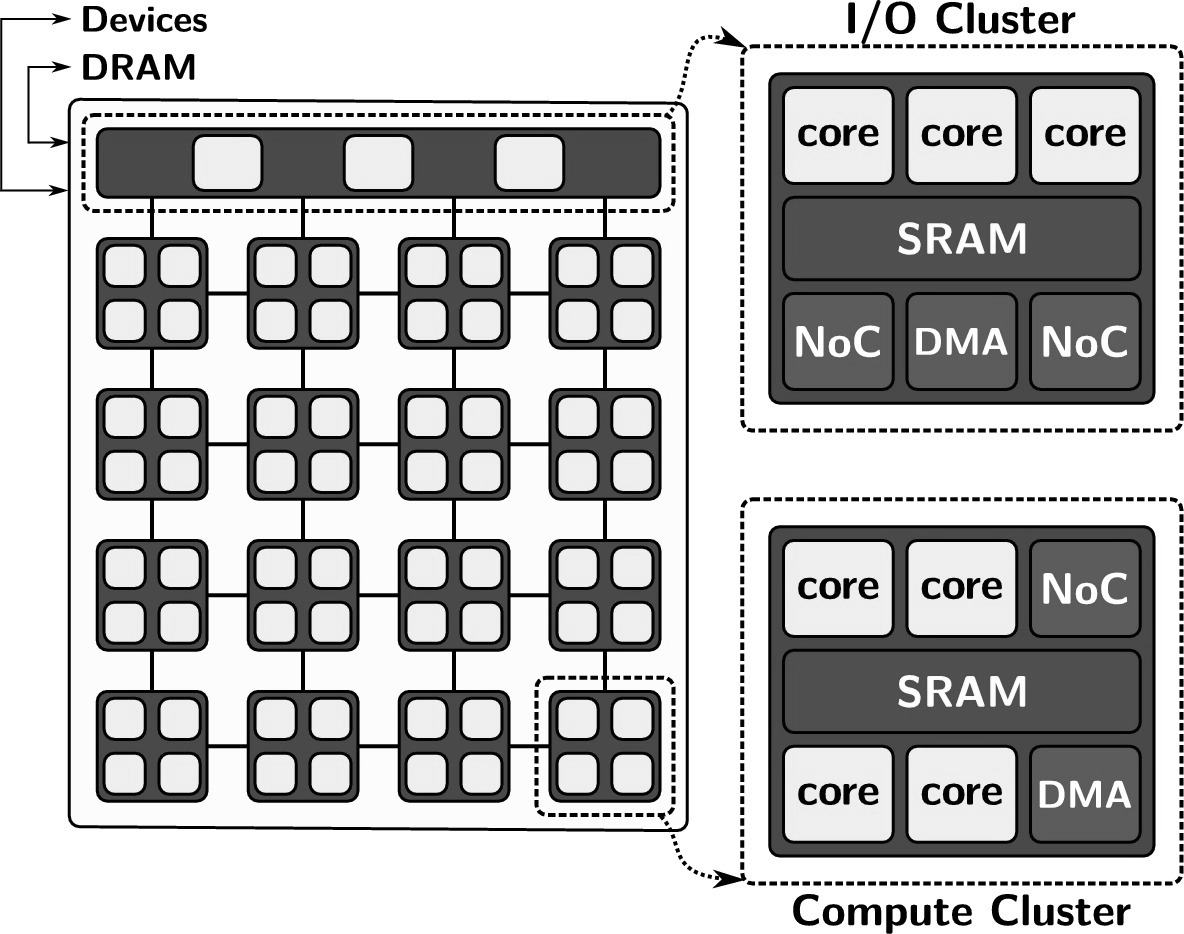
\includegraphics[width=0.5\linewidth]{content/images/lw-overview-gs.jpg}
    \fonte{\citeonline{penna2021inter}}
    \label{fig.lw-overview}
\end{figure}

Apesar dos processadores \lws serem uma alternativa às abordagens tradicionais no que se refere ao aumento de desempenho, as características arquiteturais introduzem severos problemas de programabilidade ao desenvolvimento de \software de aplicações paralelas~\cite{Castro-PARCO:2016}. Entre eles, podemos citar:

\begin{enumerate}[label= (\roman*)]
    \item Necessidade do uso de um modelo de programação híbrida que força troca de informação entre os \clusters exclusivamente por troca de mensagens via \noc enquanto a comunicação interna em um \cluster ocorre sobre memória compartilhada~\cite{kelly2013};
    \item Presença de um sistema de memória distribuída restritivo, formado por múltiplos espaços de endereçamento, o que exige o particionamento do conjunto de dados em blocos pequenos para manipulação nas pequenas memórias locais. A manipulação deve ocorrer um bloco de cada vez, necessitando a troca explicita de blocos com uma memória remota~\cite{Castro-PARCO:2016};
    % \item Maiores latências e gargalos de comunicação através da \noc comparado com comunicação em memória compartilhada;
    \item Falta de suporte de coerência de \cache em \hardware visando a economia de energia. Exigindo do programador a gerência da \cache via \software~\cite{francesquini2015}; e
    \item Configuração heterogênea do \hardware, como \clusters destinados a funcionalidades específicas (computação útil e I/O), o que dificulta o desenvolvimento de aplicações~\cite{barbalace2015popcorn}.
\end{enumerate}

Atualmente, estudos exploram soluções para amenizar o impacto arquiteturais sobre o desenvolvimento de \software. \oss distribuídos destacam-se por proverem um ambiente de programação mais robusto e rico~\cite{asmussen_m3:_2016, kluge_operating_2014, penna:sbesc19}. Dentre essas soluções, o modelo de um \os distribuído baseado em uma abordagem \multikernel, o \nanvix, destaca-se por aderir a natureza distribuída e restritiva dos \lws~\cite{penna2017-2,penna2019}.

Apesar do \nanvix ser uma solução promissora para o desenvolvimento de \software em \lws, a maneira como o \os é estruturado atualmente ainda pode ser melhorada. O mecanismo de gerenciamento de processos dificulta a mobilidade dos processos dentro do processador, já que o processo passa todo seu ciclo de vida em um mesmo \cluster. Isso significa que a partir do momento em que o processo inicia a execução em um \cluster, ele fará todo seu trabalho computacional e finalizará a execução no mesmo \cluster. Isso afeta negativamente o desempenho do sistema pois impede o remanejamento dos processos sob demanda para melhor aproveitamento dos recursos disponíveis. Por exemplo, alocar processos que se comunicam intensamente em \clusters próximos reduz a latência de comunicação e aumenta o desempenho da aplicação~\cite{vanz2022virtualizaccao}.

Neste cenário, a virtualização dos recursos do processador é importante para o suporte a multi-aplicação, melhor uso do \hardware disponível e aumento da mobilidade dos processos~\cite{vanz2022virtualizaccao}. Contudo, as características arquiteturais dos \lws, especialmente relacionadas à memória, inviabilizam um suporte complexo para virtualização. Por exemplo, máquinas virtuais utilizadas em ambientes \cloud possuem à disposição centenas de GBs de memória para isolar duplicatas inteiras do \os com a ajuda de virtualização a nível de instrução~\cite{sharma2016containers}. Nos \lws, as pequenas memórias locais e a simplificação do \hardware para reduzir o consumo energético restringem os tipos de virtualização suportados.

Neste contexto, este trabalho explora um modelo mais leve de virtualização para \lws baseado no conceito de contêineres. Contêineres são executados pelo \os como aplicações virtuais e não incluem um \os convidado, resultando em um menor impacto no sistema de memória e requisitando menor complexidade do \hardware~\cite{thalheim2018cntr, sharma2016containers}.

\section{Objetivos}
\label{sec.goals}

Com base nas motivações citadas previamente, os objetivos deste trabalho serão especificados nas próximas seções.

\subsection{Objetivo Principal}
\label{sec.goals.primary}

O objetivo principal deste trabalho é virtualizar os recursos internos de um \cluster de um \lw. Ao desvincular os recursos locais utilizados por um processo dentro do \nanvix, um \os distribuído para \lws, conseguimos prover maior controle e mobilidade de processos no processador.

\subsection{Objetivos Específicos}
\label{sec.goals.secondary}

\begin{enumerate}[label= (\roman*)]
    \item Explorar e implementar um modelo de virtualização baseado em contêineres no \nanvix;
    \item Explorar e implementar um modelo de migração de processos no \nanvix utilizando a abordagem de virtualização com contêineres;
    \item Analisar o impacto do modelo de virtualização no \nanvix;
    \item Analisar a corretude, eficiência e impacto da migração de processos  através do desenvolvimento de testes e experimentos;
\end{enumerate}

\section{Contribuições}
Esse trabalho de conclusão propõe o suporte à virtualização e migração de processos no \nanvix. A parte inicial deste trabalho foi publicado na \erad e recebeu o prêmio Aurora Cera de melhor artigo do Fórum de Iniciação Científica~\cite{vanz2022virtualizaccao}.

\section{Organização do Trabalho}
\label{sec.organization}

Os próximos capítulos deste trabalho estão organizadas da seguinte maneira. O \autoref{chap.background} apresenta conceitos fundamentais para o entendimento do trabalho, tais como um detalhamento sobre virtualização, migração de processos e um aprofundamento sobre a arquitetura dos \lws e do \nanvix. O \autoref{chap.related-work} discute os trabalhos relacionados. O \autoref{chap.dev.virtualizacao} expõe a proposta deste trabalho de conclusão de curso e os detalhes de desenvolvimento da solução. O \autoref{chap.experiment-methodology} exibe como ocorreu a tomada de decisão sobre o que avaliar e como os testes foram feitos. Os resultados experimentais são exibidos e discutidos no \autoref{chap.results}. Por fim, o \autoref{chap.conclusions} apresenta as conclusões deste trabalho e pontua os próximos passos da pesquisa.
